
\section{Intelligent Annotation}
\label{sec:annotation}

Here we describe our annotation process.  Each document is a single quiz bowl
question containing an average of 5.2 sentences.  While quiz bowl covers all
areas of academic knowledge, we focus on questions about literature from
\newcite{boyd-graber-12}, as annotation standards are more straightforward.

Our webapp (Figure~\ref{fig:screenshot}) allows users to annotate a question by
highlighting a phrase using their mouse and then pressing a number corresponding
to the coreference group to which it belongs. Each group is highlighted with a
single color in the interface. The webapp displays a single question at a time,
and for some questions, users can compare their answers against gold annotations by the authors.
We provide annotators the ability to see if their tags match the gold labels for a few documents
as we need to provide a mechanism to help them learn the annotation guidelines as the annotators are crowdsourced volunteers.
This improves inter-annotator agreement.

The webapp was advertised to quiz bowl players before a national tournament and
attracted passionate, competent annotators preparing for the tournament. A
leaderboard was implemented to encourage competitiveness, and prizes were given
to the top five annotators.

Users are instructed to annotate all authors, characters, works, and the answer
to the question (even if the answer is not one of the previously specified types
of entities).  We consider a coreference to be the maximal span that can be
replaced by a pronoun.\footnote{We phrased the instruction in this way to allow
  our educated but linguistically unsavvy annotators to approximate a noun
  phrase.} As an example, in the phrase \emph{this folk sermon by James Weldon
  Johnson}, the entire phrase is marked, not just \emph{sermon} or \emph{this
  folk sermon}. Users are asked to consider appositives as separate coreferences
to the same entity. Thus, \emph{The Japanese poet Basho} has two phrases to be
marked, \emph{The Japanese poet} and \emph{Basho}, which both refer to the same
group.\footnote{The datasets, full annotation guide, and code can be found
  at~\url{http://www.cs.umd.edu/~aguha/qbcoreference}.} Users annotated
prepositional phrases attached to a noun to capture entire noun phrases.

Titular mentions are mentions that refer to entities with similar names or the
same name as a title, e.g., ``The titular doctor'' refers to the person
``Dr. Zhivago'' while talking about the book with the same name. For our purposes, all titular mentions refer to the same coreference group. We also encountered a few mentions that refer to multiple groups; for example, in the sentence \emph{Romeo met Juliet at a fancy ball, and they get married the next day}, the word \emph{they} refers to both \emph{Romeo} and \emph{Juliet}. Currently, our webapp cannot handle such mentions.

To illustrate how popular the webapp proved to be among the quiz bowl community,
we had 615 documents tagged by seventy-six users within a month.  The top five
annotators, who between them tagged 342 documents out of 651, have an agreement
rate of 87\% with a set of twenty author-annotated questions used to measure
tagging accuracy.

We only consider documents that have either been tagged by four or more users with
a predetermined degree of similarity and verified by one or more
author (150 documents), or documents tagged
by the authors in committee (250 documents). Thus,
our gold dataset has 400 documents.

\begin{figure*}[t!]
  \centering
  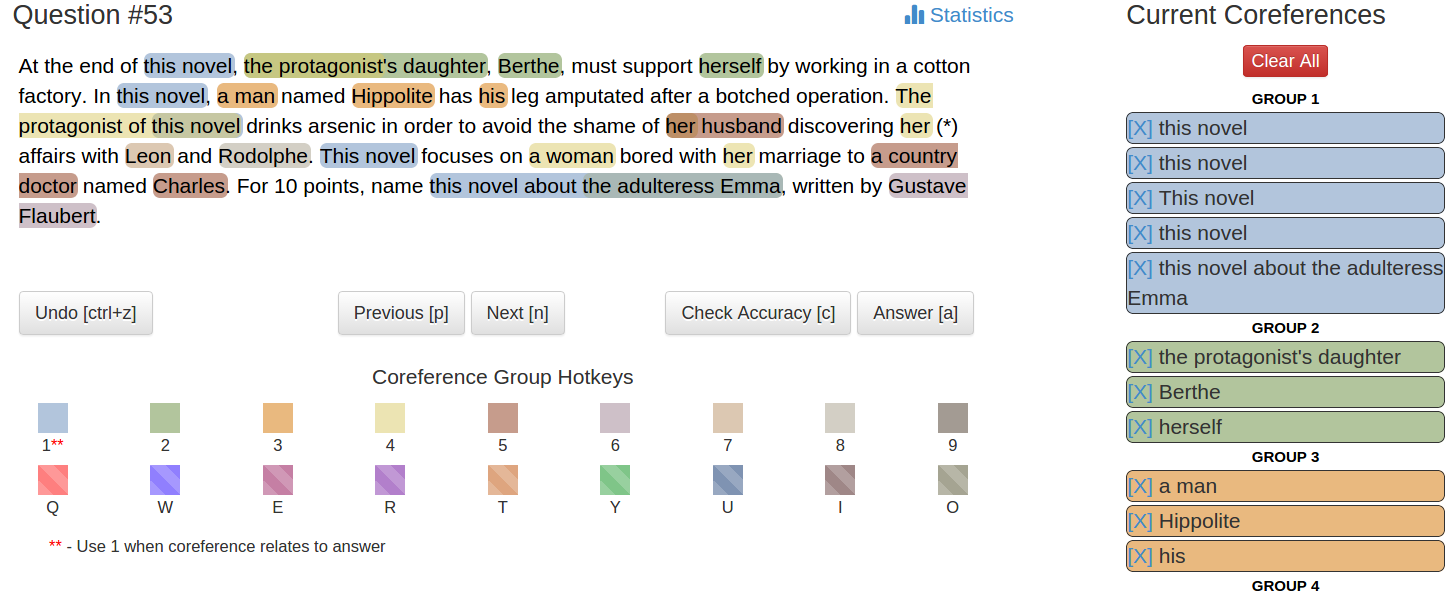
\includegraphics[scale=0.31]{2015_naacl_qb_coref/figures/webapp.png}
  \caption{The webapp to collect annotations. The user highlights
    a phrase and then assigns it to a group (by number).
    Showing a summary list of coreferences on the right significantly speeds up user
    annotations.}
  \label{fig:screenshot}
\end{figure*}

\begin{table}
\begin{center}
\begin{tabular}{lcc}
\hline
\textbf{Number of \dots} & \textbf{Quiz bowl} & \textbf{OntoNotes}\\
\hline
\textbf{documents}\tablefootnote{This number is for the OntoNotes training split only.} & 400 & 1,667\\
\textbf{sentences} & 1,890 & 44,687\\
\textbf{tokens} & 50,347 & 955,317\\
\textbf{mentions} & 9,471 & 94,155\\
\textbf{singletons}\tablefootnote{OntoNotes is not annotated for singletons.} & 2,461 & 0\\
\textbf{anaphora} & 7,010 & 94,155\\
\textbf{nested ment.} & 2,194 & 11,454\\

\hline
\end{tabular}
\caption{Statistics of both our quiz bowl dataset and the OntoNotes training
  data from the \conll{} 2011 shared task.}
\label{table2}
\end{center}
\end{table}

Both our quiz bowl dataset and the OntoNotes dataset are summarized in
Table~\ref{table2}. If coreference resolution is done by pairwise
classification, our dataset has a total of 116,125 possible mention pairs. On
average it takes about fifteen minutes to tag a document because often the
annotator will not know which mentions co-refer to what group without using
external knowledge. OntoNotes is 18.97 larger than our dataset in terms of
tokens but only 13.4 times larger in terms of mentions.\footnote{These numbers
  do not include singletons as OntoNotes does not have them tagged, while ours
  does.} Next, we describe a technique that
allows our webapp to choose which documents to display for annotation.

\subsection{Active Learning}
\label{sec:al}




\emph{Active learning} is a technique that alternates between training and
annotation by selecting instances or documents that are maximally useful for a
classifier~\cite{settles2010active}. Because of the large sample space and amount of diversity
present in the data, active learning helps us build our coreference dataset. To be more concrete, the original corpus contains over
7,000 literature questions, and we want to tag only the useful ones. Since it can take a quarter hour to tag a single document and we want
at least four annotators to agree on every document that we include in the final dataset, annotating all 7,000 questions
is infeasible.

We follow \newcite{miller2012active}, who use active learning for document-level
coreference rather than at the mention level. Starting from a seed set of a
hundred documents and an evaluation set of fifty documents\footnote{These were
  documents tagged by the quiz bowl community, so we didn't have to make them
  wait for the active learning process to retrain candidate models.} we sample
250 more documents from our set of 7,000 quiz bowl questions. We use the
Berkeley coreference system (described in the next section) for the training
phase. In Figure~\ref{fig:al} we show the effectiveness of our iteration
procedure. Unlike the result shown by \newcite{miller2012active}, we find that
for our dataset voting sampling beats random sampling, which supports the
findings of~\newcite{laws2012active}.

Voting sampling works by dividing the seed set into multiple parts and using each
to train a model. Then, from the rest of the dataset we select the document that has the most
variance in results after predicting using all of the models. Once that document gets tagged, we add it to the seed set, retrain, and repeat the procedure. This process is
impractical with instance-level active learning methods, as there are 116,125 mention pairs (instances) for just 400 documents. Even with document-level sampling, the procedure of training on all
documents in the seed set and then testing every document in the sample space is
a slow task. Batch learning can speed up this process at the cost of increased document redundancy; we choose not to use it because we want a diverse collection of annotated documents.
\begin{figure}[t!]
  \centering
  \includegraphics[width=\linewidth]{2015_naacl_qb_coref/auto_fig/active}
  \caption{Voting sampling active learning works better than randomly sampling for annotation.}
  \label{fig:al}
\end{figure}
Active learning's advantage is that new documents are more likely to contain diverse (and thus interesting) combinations of entities and references, which annotators noticed during the annotation process. Documents selected by the active learning process were dissimilar to previously-selected questions in both content and structure.